\section{Introduction}

Consider choosing a restaurant for a friend. Months ago, she said, ``I do not eat seafood, and I am cutting back on spicy food for now.'' Last week, she added, ``I am eating spicy food again.'' Recalling only ``dietary restrictions'' loses which preference changed; remembering only the latest message loses the seafood restriction. A useful recollection connects both conversations to the same person, distinguishes what changed from what still applies, and preserves qualifiers such as ``for now'' and ``cutting back.''

An agent faces the same problem across a growing history. It needs a compact way to locate related episodes without discarding the details that determine a future answer. A fixed summary may omit such details before the question is known; rereading the entire history makes each query pay for irrelevant context. Deep-Dream separates finding relevant memories from reading the evidence needed to answer.

% Figure 1: first-page evidence-path motivation
\begin{figure}[h]
  \centering
  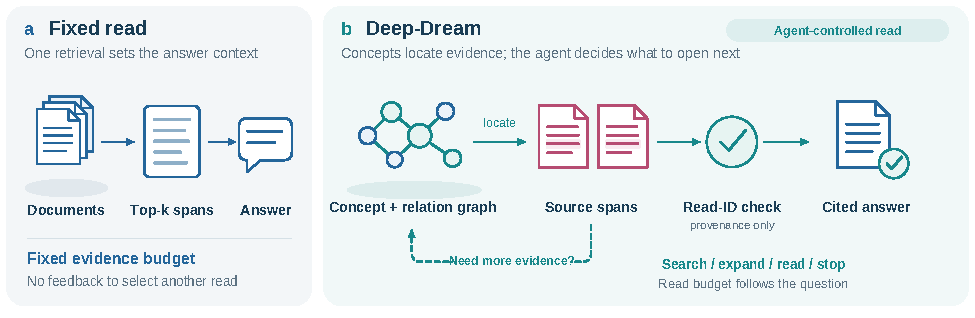
\includegraphics[width=0.98\columnwidth]{figures/fig0_motivation.pdf}
  \caption{Separating navigation from evidence. Deep-Dream first locates candidate source text and then lets the agent read, verify, or stop within a budget.}
  \label{fig:motivation}
\end{figure}

We define Deep-Dream as a \emph{document-first temporal concept graph for agentic long-term memory}. The definition has three parts.

\begin{itemize}
    \item \textbf{Documents are the authority.} Original files, episodes, and exact source spans are retained. Concepts and relations point to this material; they do not replace it with a fact that the system is allowed to treat as true.
    \item \textbf{Observation time is the state axis.} Each processed input adds an observation and, when needed, a new version. Earlier observations can still be found. Event dates may be part of the observed text, but they do not create a second graph state timeline.
    \item \textbf{The graph is a navigation layer.} Stable concept families, relation edges, and version links narrow the search space. They answer \textquotedblleft where should the agent look next?\textquotedblright; the source span answers \textquotedblleft what was actually written?\textquotedblright
\end{itemize}

The same separation shapes construction and use. At write time, a low-confidence match is kept as a provisional family instead of forcing an irreversible merge. For example, an early note may say only "Alex approved the contract." If the corpus contains a lab Alex and a vendor Alex, the system keeps two candidate families. Later notes such as "Alex from the lab presented with Dr. Liu" and "the vendor Alex renewed the account" add organization and relation evidence, so compatible pointers can be redirected without editing either source span. An eager merge would make a query about one Alex retrieve the other person's contract and project facts. At read time, the agent can follow a concept, expand a relation neighborhood, open an episode, and return to the source span. A citation check accepts only source identifiers returned by the current read path.

The two write implementations differ in when an entity identity becomes final. The initial implementation (Base) commits an identity as each window arrives. The revised implementation (Align+) first records the observation and candidate matches, then merges compatible identities after the surrounding evidence has been processed. Both build the same kind of graph.

These design choices yield five predictions. Step-by-step source reading should help when an answer requires several mentions or a later correction. Observation times and version links should keep earlier and later evidence available together. Concept and relation links should connect evidence spread across episodes for multi-hop questions. An append-only store should fail when a stored fact must be deleted or treated as absent. Delaying identity decisions should reduce duplicate families and ingest cost, even if it does not improve every accuracy score.

Four benchmarks target distinct abilities. MemoryAgentBench keeps the questions and memory collection fixed while comparing one fixed retrieval result, repeated calls to read-only memory tools, and direct reading of source files with citation checks. LongMemEval writes complete conversations before testing whether an older statement and a later correction can be found together. LoCoMo reports binary $J$, the average of 1/0 correctness judgments, for single-hop, multi-hop, temporal, and open-domain questions. MEME tests deleted facts, facts linked to deleted items, and facts that were never present. Matched runs compare the two write implementations.

The paper makes four contributions:
\begin{itemize}
    \item \textbf{A memory representation.} A document-first memory state $M_t=(F_t,O_t,G_t)$ separates stable concept families, append-only observations, and relation/version links.
    \item \textbf{A step-by-step reading method.} An agent controls concept search, relation expansion, source reading, verification, and stopping; the citation check ensures that cited text was actually opened.
    \item \textbf{An information-theoretic account.} Delayed identity alignment, the search/evidence decomposition, and query-time reading budgets are related to conditional information and rate--distortion, with assumptions and non-claims stated explicitly.
    \item \textbf{An evaluation across four memory tasks.} MAB, LongMemEval, LoCoMo, and MEME expose both strengths and failures across retrieval, temporal access, multi-hop linking, and deletion.
\end{itemize}

